\subsubsection{Dinâmica do manipulador}
A dinâmica de um manipulador robótico é a análise de velocidades, acelerações e
torques das juntas. Para esta análise, assume-se que o efetuador, pistola de
revestimento, possui velocidade 40m/min constante em todos os pontos amostrados
da pá. Como velocidades e acelerações exigem a computação de derivadas, é
realizada uma melhor discretização da pá da turbina, na qual o passo de
amostragem é menor e um filtro garante espaçamento uniforme dos pontos de 10 mm.
Para um lado da pá, são amostrados, portanto, 130 mil pontos.

Para cada ponto amostrado da pá, faz-se a análise cinemática e são armazenados
os pontos que são possíveis de serem revestidos, como na
seção~\ref{sec::cinematica}, isto é, são armazenados os pontos que possuem
solução de cinemática inversa. Posteriormente, para cada ponto revestido, é
criado um conjunto contendo seus 8 pontos vizinhos através de um algoritmo k-d
tree, como na figura~\ref{fig::pontosdin}, onde $p_r$ é o ponto de referência a
ser analisado dinamicamente e os pontos ${p_1,p_2,q_1,q_2,r_1,r_2,s_1,s_2}$ são auxiliares
para o estudo. 

\begin{figure}[h!]	
	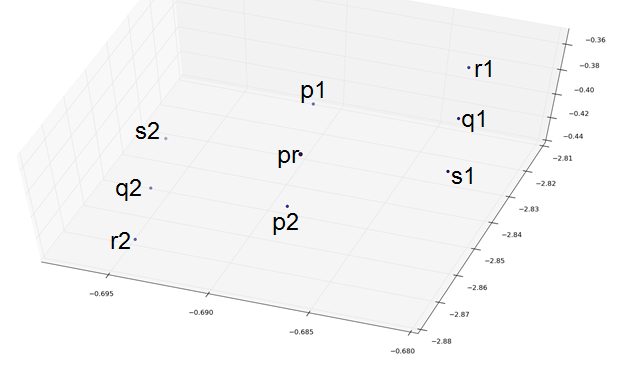
\includegraphics[width=\columnwidth]{figs/dinamica/pontosdinamica.png}
	\caption{Pontos exemplo amostrados da pá.}
	\label{fig::pontosdin}
\end{figure}

%As soluções de cinemática inversa (ângulos das juntas do robô)
%$\Theta_r
%=
%{\theta_{p_r},\theta_{p_1},\theta_{p_2},\theta_{q_1},\theta_{q_2},\theta_{r_1},\theta_{r_2},\theta_{s_1},\theta_{s_2}}$
As velocidades angulares das juntas são calculadas a partir da cinemática
diferencial. Para isso, usa-se o cálculo da matriz jacobiana ($J$), que é a
diferenciação (derivadas parciais) da matriz de cinemática direta em função das
variáveis de junta \citep{sciavicco2000differential}. A velocidade do efetuador
($\dot{X}$) e o jacobiano são conhecidos em cada ponto de referência, logo
podem-se calcular as velocidades das juntas do manipulador entre o ponto de
referência e cada ponto auxiliar: $\dot{X} = J\dot{q}\Rightarrow
J^+\dot{X}=\dot{q}$, onde $J^+$ é a pseudo inversa Moore-Penrose de $J$.

As velocidades angulares são $\Omega_r
=
{\omega_{p_r,p_1},\omega_{p_r,p_2},\omega_{p_r,q_1},\omega_{p_r,q_2},\omega_{p_r,r_1},\omega_{p_r,r_2},\omega_{p_r,s_1},\omega_{p_r,s_2}}$,
onde $\omega$, $\omega\in\Omega_r$, é um vetor $n \times 1$, e $n$ é o número de
juntas do robô. As velocidades dos ângulos das juntas é uma informação importate para a
verificação da viabilidade das trajetórias do robô. Para o caso do robô
MH12, onde $\omega_{\textbf{max}}={220, 200, 220, 410, 410, 610}^o/s$, por
exemplo, caso não haja $\omega\in\Omega_r$, tal que
$\omega\leq\omega_{\textbf{max}}$, não é possível realizar o revestimento do
ponto de referência $p_r$. Se $\exists \omega\in\Omega_r$ tal que
$\omega\leq\omega_{\textbf{max}}$, o ponto de referência é viável pela
cinemática inversa e pela cinemática diferencial, mas pode ser inviável ainda
pela análise dinâmica, que considera as acelerações, massas e forças do
conjunto.
